\documentclass[]{article}
\usepackage{lmodern}
\usepackage{amssymb,amsmath}
\usepackage{ifxetex,ifluatex}
\usepackage{fixltx2e} % provides \textsubscript
\ifnum 0\ifxetex 1\fi\ifluatex 1\fi=0 % if pdftex
  \usepackage[T1]{fontenc}
  \usepackage[utf8]{inputenc}
\else % if luatex or xelatex
  \ifxetex
    \usepackage{mathspec}
  \else
    \usepackage{fontspec}
  \fi
  \defaultfontfeatures{Ligatures=TeX,Scale=MatchLowercase}
\fi
% use upquote if available, for straight quotes in verbatim environments
\IfFileExists{upquote.sty}{\usepackage{upquote}}{}
% use microtype if available
\IfFileExists{microtype.sty}{%
\usepackage{microtype}
\UseMicrotypeSet[protrusion]{basicmath} % disable protrusion for tt fonts
}{}
\usepackage[margin=1in]{geometry}
\usepackage{hyperref}
\hypersetup{unicode=true,
            pdftitle={Question 5},
            pdfborder={0 0 0},
            breaklinks=true}
\urlstyle{same}  % don't use monospace font for urls
\usepackage{color}
\usepackage{fancyvrb}
\newcommand{\VerbBar}{|}
\newcommand{\VERB}{\Verb[commandchars=\\\{\}]}
\DefineVerbatimEnvironment{Highlighting}{Verbatim}{commandchars=\\\{\}}
% Add ',fontsize=\small' for more characters per line
\usepackage{framed}
\definecolor{shadecolor}{RGB}{248,248,248}
\newenvironment{Shaded}{\begin{snugshade}}{\end{snugshade}}
\newcommand{\AlertTok}[1]{\textcolor[rgb]{0.94,0.16,0.16}{#1}}
\newcommand{\AnnotationTok}[1]{\textcolor[rgb]{0.56,0.35,0.01}{\textbf{\textit{#1}}}}
\newcommand{\AttributeTok}[1]{\textcolor[rgb]{0.77,0.63,0.00}{#1}}
\newcommand{\BaseNTok}[1]{\textcolor[rgb]{0.00,0.00,0.81}{#1}}
\newcommand{\BuiltInTok}[1]{#1}
\newcommand{\CharTok}[1]{\textcolor[rgb]{0.31,0.60,0.02}{#1}}
\newcommand{\CommentTok}[1]{\textcolor[rgb]{0.56,0.35,0.01}{\textit{#1}}}
\newcommand{\CommentVarTok}[1]{\textcolor[rgb]{0.56,0.35,0.01}{\textbf{\textit{#1}}}}
\newcommand{\ConstantTok}[1]{\textcolor[rgb]{0.00,0.00,0.00}{#1}}
\newcommand{\ControlFlowTok}[1]{\textcolor[rgb]{0.13,0.29,0.53}{\textbf{#1}}}
\newcommand{\DataTypeTok}[1]{\textcolor[rgb]{0.13,0.29,0.53}{#1}}
\newcommand{\DecValTok}[1]{\textcolor[rgb]{0.00,0.00,0.81}{#1}}
\newcommand{\DocumentationTok}[1]{\textcolor[rgb]{0.56,0.35,0.01}{\textbf{\textit{#1}}}}
\newcommand{\ErrorTok}[1]{\textcolor[rgb]{0.64,0.00,0.00}{\textbf{#1}}}
\newcommand{\ExtensionTok}[1]{#1}
\newcommand{\FloatTok}[1]{\textcolor[rgb]{0.00,0.00,0.81}{#1}}
\newcommand{\FunctionTok}[1]{\textcolor[rgb]{0.00,0.00,0.00}{#1}}
\newcommand{\ImportTok}[1]{#1}
\newcommand{\InformationTok}[1]{\textcolor[rgb]{0.56,0.35,0.01}{\textbf{\textit{#1}}}}
\newcommand{\KeywordTok}[1]{\textcolor[rgb]{0.13,0.29,0.53}{\textbf{#1}}}
\newcommand{\NormalTok}[1]{#1}
\newcommand{\OperatorTok}[1]{\textcolor[rgb]{0.81,0.36,0.00}{\textbf{#1}}}
\newcommand{\OtherTok}[1]{\textcolor[rgb]{0.56,0.35,0.01}{#1}}
\newcommand{\PreprocessorTok}[1]{\textcolor[rgb]{0.56,0.35,0.01}{\textit{#1}}}
\newcommand{\RegionMarkerTok}[1]{#1}
\newcommand{\SpecialCharTok}[1]{\textcolor[rgb]{0.00,0.00,0.00}{#1}}
\newcommand{\SpecialStringTok}[1]{\textcolor[rgb]{0.31,0.60,0.02}{#1}}
\newcommand{\StringTok}[1]{\textcolor[rgb]{0.31,0.60,0.02}{#1}}
\newcommand{\VariableTok}[1]{\textcolor[rgb]{0.00,0.00,0.00}{#1}}
\newcommand{\VerbatimStringTok}[1]{\textcolor[rgb]{0.31,0.60,0.02}{#1}}
\newcommand{\WarningTok}[1]{\textcolor[rgb]{0.56,0.35,0.01}{\textbf{\textit{#1}}}}
\usepackage{graphicx,grffile}
\makeatletter
\def\maxwidth{\ifdim\Gin@nat@width>\linewidth\linewidth\else\Gin@nat@width\fi}
\def\maxheight{\ifdim\Gin@nat@height>\textheight\textheight\else\Gin@nat@height\fi}
\makeatother
% Scale images if necessary, so that they will not overflow the page
% margins by default, and it is still possible to overwrite the defaults
% using explicit options in \includegraphics[width, height, ...]{}
\setkeys{Gin}{width=\maxwidth,height=\maxheight,keepaspectratio}
\IfFileExists{parskip.sty}{%
\usepackage{parskip}
}{% else
\setlength{\parindent}{0pt}
\setlength{\parskip}{6pt plus 2pt minus 1pt}
}
\setlength{\emergencystretch}{3em}  % prevent overfull lines
\providecommand{\tightlist}{%
  \setlength{\itemsep}{0pt}\setlength{\parskip}{0pt}}
\setcounter{secnumdepth}{0}
% Redefines (sub)paragraphs to behave more like sections
\ifx\paragraph\undefined\else
\let\oldparagraph\paragraph
\renewcommand{\paragraph}[1]{\oldparagraph{#1}\mbox{}}
\fi
\ifx\subparagraph\undefined\else
\let\oldsubparagraph\subparagraph
\renewcommand{\subparagraph}[1]{\oldsubparagraph{#1}\mbox{}}
\fi

%%% Use protect on footnotes to avoid problems with footnotes in titles
\let\rmarkdownfootnote\footnote%
\def\footnote{\protect\rmarkdownfootnote}

%%% Change title format to be more compact
\usepackage{titling}

% Create subtitle command for use in maketitle
\newcommand{\subtitle}[1]{
  \posttitle{
    \begin{center}\large#1\end{center}
    }
}

\setlength{\droptitle}{-2em}

  \title{Question 5}
    \pretitle{\vspace{\droptitle}\centering\huge}
  \posttitle{\par}
    \author{}
    \preauthor{}\postauthor{}
    \date{}
    \predate{}\postdate{}
  

\begin{document}
\maketitle

\(\;\) \(\;\)

Read in the data and filter for only Californians and use
\texttt{people\_fully\_vaccinated} to forecast.

\begin{Shaded}
\begin{Highlighting}[]
\NormalTok{covid19 <-}\StringTok{ }\KeywordTok{read.csv}\NormalTok{(}\DataTypeTok{file =} \StringTok{"us_state_vaccinations.csv"}\NormalTok{, }\DataTypeTok{header =} \OtherTok{TRUE}\NormalTok{)}

\NormalTok{covid19 <-}\StringTok{ }\NormalTok{covid19[covid19[}\StringTok{'location'}\NormalTok{] }\OperatorTok{==}\StringTok{ 'California'}\NormalTok{, }\StringTok{'people_fully_vaccinated'}\NormalTok{]}
\end{Highlighting}
\end{Shaded}

\(\;\)

Fill NA's with latest non-NA value.

\begin{Shaded}
\begin{Highlighting}[]
\KeywordTok{library}\NormalTok{(}\StringTok{"zoo"}\NormalTok{)}
\NormalTok{covid19 <-}\StringTok{ }\KeywordTok{na.locf}\NormalTok{(covid19)}
\end{Highlighting}
\end{Shaded}

\(\;\)

Divide the data into a training set (first 66 days) and testing set
(last 5 days). Provided is a time series plot of the data with training
and test sets in different colours.

\begin{Shaded}
\begin{Highlighting}[]
\NormalTok{covid19 =}\StringTok{ }\KeywordTok{as.numeric}\NormalTok{(}\KeywordTok{unlist}\NormalTok{(covid19))}
\NormalTok{covid.training <-}\StringTok{ }\KeywordTok{head}\NormalTok{(covid19, }\DecValTok{66}\NormalTok{)}
\NormalTok{covid.test <-}\StringTok{ }\KeywordTok{tail}\NormalTok{(covid19, }\DecValTok{5}\NormalTok{)}

\KeywordTok{plot}\NormalTok{(covid.training,}
     \DataTypeTok{main =} \StringTok{"Fully Vaccinated Californians"}\NormalTok{,}
     \DataTypeTok{xlab =} \StringTok{"Day"}\NormalTok{,}
     \DataTypeTok{ylab =} \StringTok{"Total Vaccinations"}\NormalTok{,}
     \DataTypeTok{xlim =} \KeywordTok{c}\NormalTok{(}\DecValTok{1}\NormalTok{, }\DecValTok{71}\NormalTok{),}
     \DataTypeTok{ylim =} \KeywordTok{c}\NormalTok{(}\DecValTok{0}\NormalTok{, }\DecValTok{5500000}\NormalTok{),}
     \DataTypeTok{type =} \StringTok{"p"}\NormalTok{,}
     \DataTypeTok{pch =} \DecValTok{19}\NormalTok{,}
     \DataTypeTok{col =} \KeywordTok{adjustcolor}\NormalTok{(}\StringTok{"darkgreen"}\NormalTok{, }\FloatTok{0.5}\NormalTok{),}
     \DataTypeTok{xaxt =} \StringTok{"n"}\NormalTok{,}
     \DataTypeTok{yaxt =} \StringTok{"n"}\NormalTok{)}

\KeywordTok{lines}\NormalTok{(}\DataTypeTok{y =}\NormalTok{ covid.test,}
      \DataTypeTok{x =} \DecValTok{67}\OperatorTok{:}\DecValTok{71}\NormalTok{,}
      \DataTypeTok{type =}\StringTok{"p"}\NormalTok{,}
      \DataTypeTok{pch =} \DecValTok{19}\NormalTok{,}
      \DataTypeTok{col =} \KeywordTok{adjustcolor}\NormalTok{(}\StringTok{"darkred"}\NormalTok{, }\FloatTok{0.5}\NormalTok{))}

\KeywordTok{axis}\NormalTok{(}\DataTypeTok{side =} \DecValTok{1}\NormalTok{, }\DataTypeTok{at =}\NormalTok{ (}\DecValTok{14}\OperatorTok{*}\DecValTok{0}\OperatorTok{:}\DecValTok{5}\NormalTok{)}\OperatorTok{+}\DecValTok{1}\NormalTok{, }\DataTypeTok{labels =} \KeywordTok{c}\NormalTok{(}\StringTok{"Jan 12"}\NormalTok{,}\StringTok{"Jan 26"}\NormalTok{,}\StringTok{"Feb 9"}\NormalTok{,}\StringTok{"Feb 23"}\NormalTok{,}\StringTok{"Mar 9"}\NormalTok{, }\StringTok{"Mar 23"}\NormalTok{))}

\KeywordTok{axis}\NormalTok{(}\DataTypeTok{side =} \DecValTok{2}\NormalTok{, }\DataTypeTok{at =}\NormalTok{ (}\DecValTok{1000000}\OperatorTok{*}\DecValTok{0}\OperatorTok{:}\DecValTok{5}\NormalTok{), }\DataTypeTok{labels =} \KeywordTok{c}\NormalTok{(}\StringTok{"0"}\NormalTok{,}\StringTok{""}\NormalTok{,}\StringTok{"2M"}\NormalTok{,}\StringTok{" "}\NormalTok{,}\StringTok{"4M"}\NormalTok{, }\StringTok{" "}\NormalTok{))}

\KeywordTok{legend}\NormalTok{(}\StringTok{"topleft"}\NormalTok{,}
       \DataTypeTok{lwd =} \DecValTok{2}\NormalTok{,}
       \DataTypeTok{bty =} \StringTok{"n"}\NormalTok{,}
       \DataTypeTok{cex =} \FloatTok{0.8}\NormalTok{,}
       \DataTypeTok{legend =} \KeywordTok{c}\NormalTok{(}\StringTok{"Jan 12 - Mar 18 (Traning data)"}\NormalTok{,}
                  \StringTok{"Mar 19 - Mar 23 (Test data)"}\NormalTok{),}
       \DataTypeTok{col =} \KeywordTok{c}\NormalTok{(}\KeywordTok{adjustcolor}\NormalTok{(}\StringTok{"darkgreen"}\NormalTok{, }\FloatTok{0.5}\NormalTok{),}
               \KeywordTok{adjustcolor}\NormalTok{(}\StringTok{"darkred"}\NormalTok{, }\FloatTok{0.5}\NormalTok{)))}
\end{Highlighting}
\end{Shaded}

\begin{center}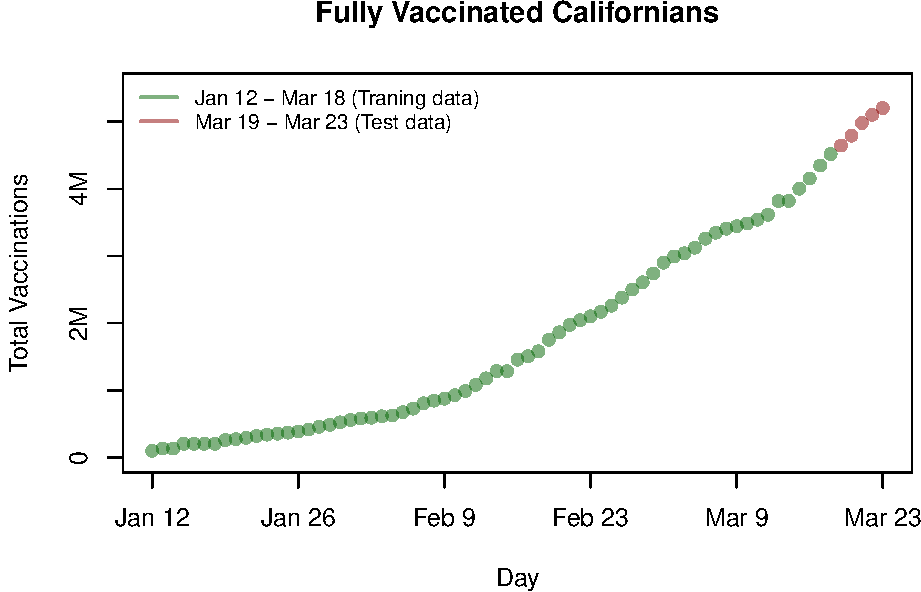
\includegraphics{Q5_files/figure-latex/unnamed-chunk-4-1} \end{center}

\(\;\)

The framework to predict when at least 50\% of Californians will be
fully vaccinated is as follows:

\begin{itemize}
\tightlist
\item
  transform non-stationary data to stationary data
\item
  fit a stationary model
\item
  forecast
\item
  add non-stationarity back
\end{itemize}

Data with a trend, change points, heteroscedasticity, or seasonality
indicate non-stationarity. From the time series plot we observe an
increasing trend and heteroscedasticity.

It is important that the variance of the series is stabilized and its
trend removed with differencing before we propose ARIMA models.

\newpage

To stabilize the variance, let's search over the grid
\textbf{\texttt{alpha=seq(-2,2,by=0.1)}} to find a value
\emph{\(\alpha\)} such that \emph{\(X = (covid19)^\alpha\)} has a
constant variance. Suppose for \(\alpha\) = 0, the transformation is
\emph{X = log(covid19)}. We bin the data into 6 segments, each
containing 11 consecutive observations, and generate a plot where the
\(x\)-axis shows the value of \(\alpha\) and the \(y\)-axis shows the
corresponding p-value of the Fligner-Kileen test of variance homogeneity
for the transformed data \emph{X}. To follow an objective method, among
the satisfactory transformations, we choose the one with the largest
p-value of Fligner's test.

\begin{Shaded}
\begin{Highlighting}[]
\CommentTok{# vector representing segment for the corresponding elements in transformed_covid19}
\NormalTok{seg <-}\StringTok{ }\KeywordTok{c}\NormalTok{(}\KeywordTok{rep}\NormalTok{(}\DecValTok{1}\OperatorTok{:}\DecValTok{6}\NormalTok{, }\DataTypeTok{each=}\DecValTok{11}\NormalTok{))}

\CommentTok{# vector to store p_values from Fligner-Kileen tests}
\NormalTok{p_values <-}\StringTok{ }\KeywordTok{c}\NormalTok{()}

\CommentTok{# vector containing values of alpha to search}
\NormalTok{alpha <-}\StringTok{ }\KeywordTok{seq}\NormalTok{(}\OperatorTok{-}\DecValTok{2}\NormalTok{,}\DecValTok{2}\NormalTok{,}\DataTypeTok{by=}\FloatTok{0.1}\NormalTok{)}

\ControlFlowTok{for}\NormalTok{ (i }\ControlFlowTok{in}\NormalTok{ alpha) \{}
  
  \CommentTok{# apply transformation}
  \ControlFlowTok{if}\NormalTok{ (i }\OperatorTok{==}\StringTok{ }\DecValTok{0}\NormalTok{) transformed_covid =}\StringTok{ }\KeywordTok{log}\NormalTok{(covid.training)}
  \ControlFlowTok{else}\NormalTok{ transformed_covid =}\StringTok{ }\NormalTok{covid.training}\OperatorTok{^}\NormalTok{i}
  
  \CommentTok{# extract p-value from test}
\NormalTok{  p_value =}\StringTok{ }\KeywordTok{fligner.test}\NormalTok{(transformed_covid, seg)}\OperatorTok{$}\NormalTok{p.value}
  
  \CommentTok{# append p-value to vector}
\NormalTok{  p_values =}\StringTok{ }\KeywordTok{c}\NormalTok{(p_values, p_value)}
  
\NormalTok{\}}

\KeywordTok{plot}\NormalTok{(}\DataTypeTok{x =}\NormalTok{ alpha, }\DataTypeTok{y =}\NormalTok{ p_values,}
     \DataTypeTok{ylab =} \StringTok{"Fligner-Kileen p-value"}\NormalTok{,}
     \DataTypeTok{main =} \StringTok{"Fligner-Kileen p-value versus Alpha"}\NormalTok{)}
\end{Highlighting}
\end{Shaded}

\begin{center}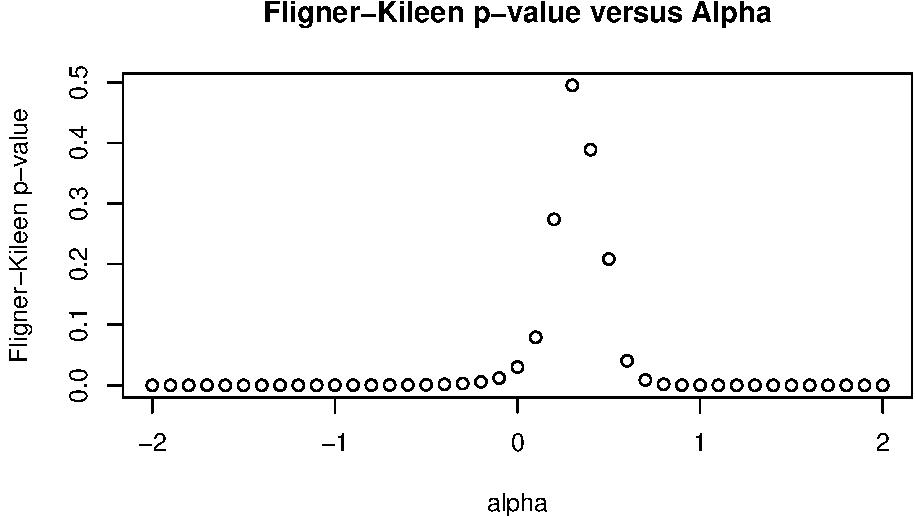
\includegraphics{Q5_files/figure-latex/unnamed-chunk-5-1} \end{center}

\begin{Shaded}
\begin{Highlighting}[]
\CommentTok{# find alpha corresponding to largest p-value}
\NormalTok{alpha[}\KeywordTok{which}\NormalTok{(p_values }\OperatorTok{==}\StringTok{ }\KeywordTok{max}\NormalTok{(p_values))]}
\end{Highlighting}
\end{Shaded}

\begin{verbatim}
## [1] 0.3
\end{verbatim}

The desired transformation is \(\alpha = 0.3\).

Provided is a time series plot of the transformed data along with the
ACF and PACF plots.

\begin{Shaded}
\begin{Highlighting}[]
\NormalTok{transformed.covid.training <-}\StringTok{ }\NormalTok{covid.training}\OperatorTok{^}\NormalTok{alpha[}\KeywordTok{which}\NormalTok{(p_values }\OperatorTok{==}\StringTok{ }\KeywordTok{max}\NormalTok{(p_values))]}

\KeywordTok{plot}\NormalTok{(transformed.covid.training,}
     \DataTypeTok{main =} \StringTok{"Transformed Time Series of Fully Vaccinated Californians"}\NormalTok{,}
     \DataTypeTok{xlab =} \StringTok{"Day"}\NormalTok{,}
     \DataTypeTok{ylab =} \StringTok{"Transformed Total Vaccinations. alpha=0.3"}\NormalTok{,}
     \DataTypeTok{xlim =} \KeywordTok{c}\NormalTok{(}\DecValTok{1}\NormalTok{, }\DecValTok{66}\NormalTok{),}
     \DataTypeTok{ylim =} \KeywordTok{c}\NormalTok{(}\DecValTok{0}\NormalTok{, }\DecValTok{100}\NormalTok{),}
     \DataTypeTok{type =} \StringTok{"p"}\NormalTok{,}
     \DataTypeTok{pch =} \DecValTok{19}\NormalTok{,}
     \DataTypeTok{col =} \KeywordTok{adjustcolor}\NormalTok{(}\StringTok{"darkgreen"}\NormalTok{, }\FloatTok{0.5}\NormalTok{),}
     \DataTypeTok{xaxt =} \StringTok{"n"}\NormalTok{)}

\KeywordTok{axis}\NormalTok{(}\DataTypeTok{side =} \DecValTok{1}\NormalTok{, }\DataTypeTok{at =}\NormalTok{ (}\DecValTok{14}\OperatorTok{*}\DecValTok{0}\OperatorTok{:}\DecValTok{5}\NormalTok{)}\OperatorTok{+}\DecValTok{1}\NormalTok{, }\DataTypeTok{labels =} \KeywordTok{c}\NormalTok{(}\StringTok{"Jan 12"}\NormalTok{,}\StringTok{"Jan 26"}\NormalTok{,}\StringTok{"Feb 9"}\NormalTok{,}\StringTok{"Feb 23"}\NormalTok{,}\StringTok{"Mar 9"}\NormalTok{, }\StringTok{"Mar 23"}\NormalTok{))}

\KeywordTok{legend}\NormalTok{(}\StringTok{"topleft"}\NormalTok{,}
       \DataTypeTok{lwd =} \DecValTok{2}\NormalTok{,}
       \DataTypeTok{bty =} \StringTok{"n"}\NormalTok{,}
       \DataTypeTok{cex =} \FloatTok{0.8}\NormalTok{,}
       \DataTypeTok{legend =} \KeywordTok{c}\NormalTok{(}\StringTok{"Jan 12 - Mar 18 (Traning data)"}\NormalTok{),}
       \DataTypeTok{col =} \KeywordTok{c}\NormalTok{(}\KeywordTok{adjustcolor}\NormalTok{(}\StringTok{"darkgreen"}\NormalTok{, }\FloatTok{0.5}\NormalTok{)))}
\end{Highlighting}
\end{Shaded}

\begin{center}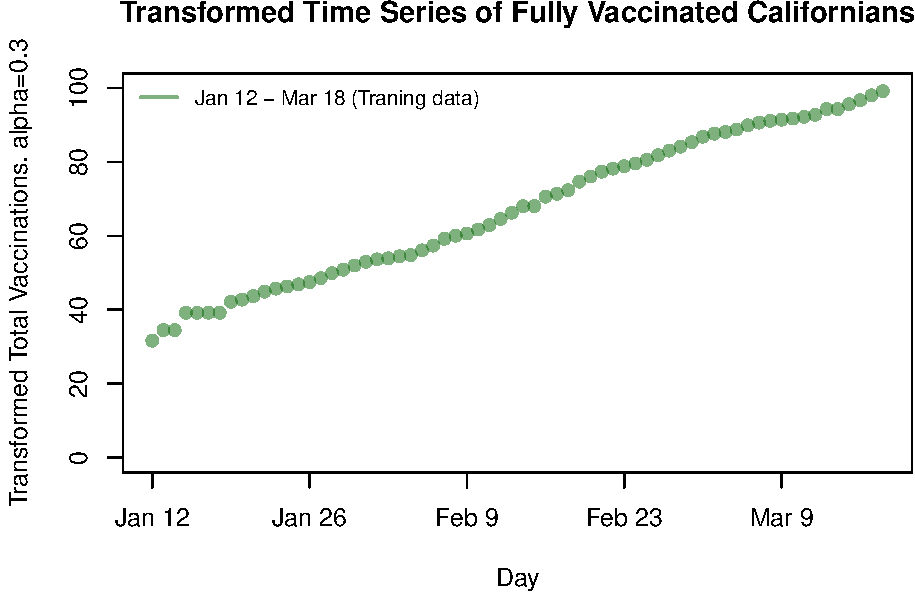
\includegraphics{Q5_files/figure-latex/unnamed-chunk-6-1} \end{center}

\begin{Shaded}
\begin{Highlighting}[]
\KeywordTok{par}\NormalTok{(}\DataTypeTok{mfrow=}\KeywordTok{c}\NormalTok{(}\DecValTok{1}\NormalTok{,}\DecValTok{2}\NormalTok{))}
\KeywordTok{acf}\NormalTok{(transformed.covid.training)}
\KeywordTok{pacf}\NormalTok{(transformed.covid.training)}
\end{Highlighting}
\end{Shaded}

\begin{center}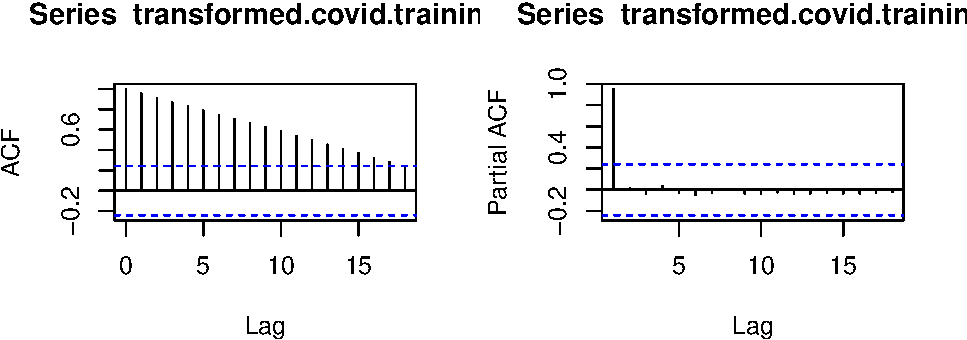
\includegraphics{Q5_files/figure-latex/unnamed-chunk-7-1} \end{center}

There is a clear increasing trend in the data and the ACF has a linear
decay that implies differencing is required to remove the trend.

\begin{Shaded}
\begin{Highlighting}[]
\NormalTok{diff.transformed.covid.training <-}\StringTok{ }\KeywordTok{diff}\NormalTok{(transformed.covid.training, }\DataTypeTok{differences=}\DecValTok{2}\NormalTok{)}

\KeywordTok{par}\NormalTok{(}\DataTypeTok{mfrow=}\KeywordTok{c}\NormalTok{(}\DecValTok{1}\NormalTok{,}\DecValTok{3}\NormalTok{))}
\KeywordTok{plot}\NormalTok{(diff.transformed.covid.training, }\DataTypeTok{type=}\StringTok{'l'}\NormalTok{)}
\KeywordTok{acf}\NormalTok{(diff.transformed.covid.training)}
\KeywordTok{pacf}\NormalTok{(diff.transformed.covid.training)}
\end{Highlighting}
\end{Shaded}

\begin{center}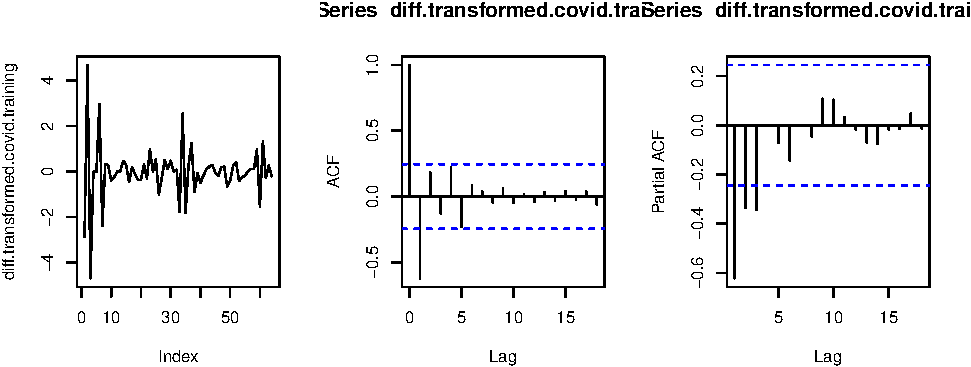
\includegraphics{Q5_files/figure-latex/unnamed-chunk-8-1} \end{center}

Up until now, we have applied a power transformation to remove the
heteroscedasticity and twice differencing to remove the trend.

Next, we propose models for the stationary data and perform full
residuals diagnostics for the proposed ARIMA models.

\begin{itemize}
\tightlist
\item
  Model 1: the ACF has an exponential decay and the PACF cuts off after
  lag 3, so we consider ARIMA(3,2,0).
\item
  Model 2: the PACF has an exponential decay and the ACF cuts off after
  lag 1, so we consider ARIMA(0,2,1).
\item
  Model 3: since in models 1 and 2 we justified exponential decay on the
  ACF and PACF, it could be exponential decay on both, so we consider
  ARIMA(1,2,1).
\end{itemize}

\newpage

\hypertarget{model-1-arima3-2-0}{%
\subsection{Model 1: ARIMA(3, 2, 0)}\label{model-1-arima3-2-0}}

\begin{Shaded}
\begin{Highlighting}[]
\KeywordTok{library}\NormalTok{(astsa)}

\NormalTok{model1 <-}\StringTok{ }\KeywordTok{sarima}\NormalTok{(transformed.covid.training, }\DataTypeTok{p=}\DecValTok{3}\NormalTok{, }\DataTypeTok{d=}\DecValTok{2}\NormalTok{, }\DataTypeTok{q=}\DecValTok{0}\NormalTok{, }\DataTypeTok{details =} \OtherTok{TRUE}\NormalTok{)}
\end{Highlighting}
\end{Shaded}

\begin{verbatim}
## initial  value -0.195944 
## iter   2 value -0.259502
## iter   3 value -0.355965
## iter   4 value -0.450607
## iter   5 value -0.452855
## iter   6 value -0.455779
## iter   7 value -0.455836
## iter   8 value -0.455842
## iter   8 value -0.455842
## final  value -0.455842 
## converged
## initial  value -0.125312 
## iter   2 value -0.182048
## iter   3 value -0.218676
## iter   4 value -0.220231
## iter   5 value -0.220533
## iter   6 value -0.220782
## iter   7 value -0.220853
## iter   8 value -0.220890
## iter   9 value -0.220892
## iter  10 value -0.220892
## iter  11 value -0.220892
## iter  12 value -0.220892
## iter  13 value -0.220892
## iter  14 value -0.220892
## iter  14 value -0.220892
## iter  14 value -0.220892
## final  value -0.220892 
## converged
\end{verbatim}

\begin{center}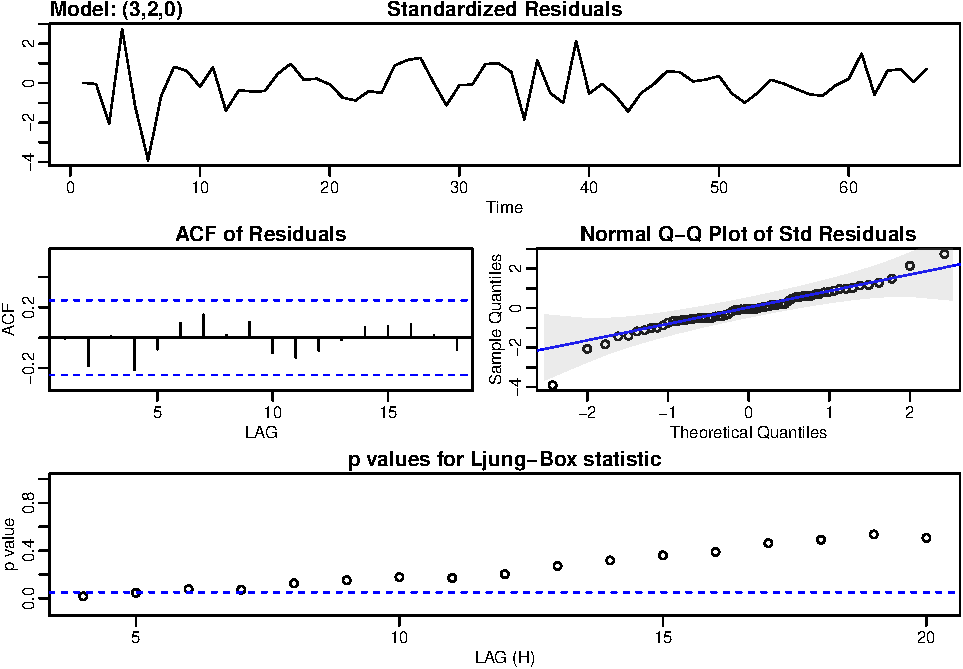
\includegraphics{Q5_files/figure-latex/unnamed-chunk-10-1} \end{center}

\begin{Shaded}
\begin{Highlighting}[]
\NormalTok{seg <-}\StringTok{ }\KeywordTok{c}\NormalTok{(}\KeywordTok{rep}\NormalTok{(}\DecValTok{1}\OperatorTok{:}\DecValTok{5}\NormalTok{, }\DataTypeTok{each=}\DecValTok{11}\NormalTok{), }\KeywordTok{rep}\NormalTok{(}\DecValTok{6}\NormalTok{,}\DecValTok{11}\NormalTok{))}
\KeywordTok{fligner.test}\NormalTok{(model1}\OperatorTok{$}\NormalTok{fit}\OperatorTok{$}\NormalTok{residuals, seg)}
\end{Highlighting}
\end{Shaded}

\begin{verbatim}
## 
##  Fligner-Killeen test of homogeneity of variances
## 
## data:  model1$fit$residuals and seg
## Fligner-Killeen:med chi-squared = 7.3465, df = 5, p-value = 0.1961
\end{verbatim}

\begin{Shaded}
\begin{Highlighting}[]
\KeywordTok{shapiro.test}\NormalTok{(model1}\OperatorTok{$}\NormalTok{fit}\OperatorTok{$}\NormalTok{residuals)}
\end{Highlighting}
\end{Shaded}

\begin{verbatim}
## 
##  Shapiro-Wilk normality test
## 
## data:  model1$fit$residuals
## W = 0.95251, p-value = 0.01316
\end{verbatim}

\(\;\)

\begin{itemize}
\tightlist
\item
  ARIMA(3, 2, 0)

  \begin{itemize}
  \tightlist
  \item
    Homoscedasticity: the time series of the residuals has no trend and
    the p-value of Fligner's test (0.1961) confirms the validity of
    homoscedasticity.
  \item
    Normality: a few points in the QQplot deviate from the straight line
    resulting in the small p-value of Shapiro-Wilk's test (0.01316).
    While the normality assumption is not quite valid, it not heavily
    violated either.
  \item
    White Noise: a few p-values of Ljung-Box statistic are below the
    threshold which raises concerns about the independence of the
    residuals.
  \end{itemize}
\end{itemize}

\newpage

\hypertarget{model-2-arima0-2-1}{%
\subsection{Model 2: ARIMA(0, 2, 1)}\label{model-2-arima0-2-1}}

\(\;\)

\begin{Shaded}
\begin{Highlighting}[]
\KeywordTok{library}\NormalTok{(astsa)}

\NormalTok{model2 <-}\StringTok{ }\KeywordTok{sarima}\NormalTok{(transformed.covid.training, }\DataTypeTok{p=}\DecValTok{0}\NormalTok{, }\DataTypeTok{d=}\DecValTok{2}\NormalTok{, }\DataTypeTok{q=}\DecValTok{1}\NormalTok{, }\DataTypeTok{details =} \OtherTok{TRUE}\NormalTok{)}
\end{Highlighting}
\end{Shaded}

\begin{verbatim}
## initial  value 0.188759 
## iter   2 value -0.105041
## iter   3 value -0.128231
## iter   4 value -0.128461
## iter   5 value -0.130250
## iter   6 value -0.130278
## iter   7 value -0.130279
## iter   7 value -0.130279
## final  value -0.130279 
## converged
## initial  value -0.165956 
## iter   2 value -0.203913
## iter   3 value -0.206846
## iter   4 value -0.207428
## iter   5 value -0.207431
## iter   6 value -0.207433
## iter   6 value -0.207433
## iter   6 value -0.207433
## final  value -0.207433 
## converged
\end{verbatim}

\begin{center}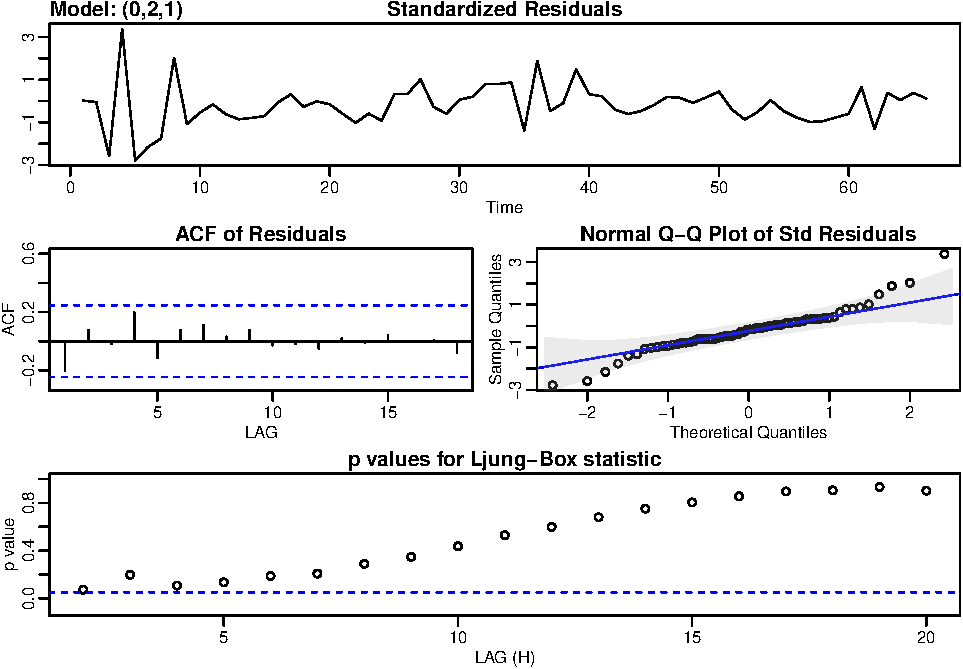
\includegraphics{Q5_files/figure-latex/unnamed-chunk-11-1} \end{center}

\begin{Shaded}
\begin{Highlighting}[]
\NormalTok{seg <-}\StringTok{ }\KeywordTok{c}\NormalTok{(}\KeywordTok{rep}\NormalTok{(}\DecValTok{1}\OperatorTok{:}\DecValTok{5}\NormalTok{, }\DataTypeTok{each=}\DecValTok{11}\NormalTok{), }\KeywordTok{rep}\NormalTok{(}\DecValTok{6}\NormalTok{,}\DecValTok{11}\NormalTok{))}
\KeywordTok{fligner.test}\NormalTok{(model2}\OperatorTok{$}\NormalTok{fit}\OperatorTok{$}\NormalTok{residuals, seg)}
\end{Highlighting}
\end{Shaded}

\begin{verbatim}
## 
##  Fligner-Killeen test of homogeneity of variances
## 
## data:  model2$fit$residuals and seg
## Fligner-Killeen:med chi-squared = 16.336, df = 5, p-value =
## 0.005947
\end{verbatim}

\begin{Shaded}
\begin{Highlighting}[]
\KeywordTok{shapiro.test}\NormalTok{(model2}\OperatorTok{$}\NormalTok{fit}\OperatorTok{$}\NormalTok{residuals)}
\end{Highlighting}
\end{Shaded}

\begin{verbatim}
## 
##  Shapiro-Wilk normality test
## 
## data:  model2$fit$residuals
## W = 0.94062, p-value = 0.003409
\end{verbatim}

\(\;\)

\begin{itemize}
\tightlist
\item
  ARIMA(0, 2, 1)

  \begin{itemize}
  \tightlist
  \item
    Homoscedasticity: the time series of the residuals has no trend but
    the p-value of Fligner's test (0.005947) raises concern. The
    constant variance assumption of the residuals is not valid.
  \item
    Normality: the points in the QQplot deviate from the straight line
    resulting in the small p-value of Shapiro-Wilk's test (0.003409).
    The normality assumption of the residuals is not valid.
  \item
    White Noise: the p-values of the Ljung-Box statistic are above the
    threshold and there is no concern in the ACF plot. We can safely
    conclude the residuals are realizations of white noise.
  \end{itemize}
\end{itemize}

\(\;\)

\hypertarget{model-3-arima1-2-1}{%
\subsection{Model 3: ARIMA(1, 2, 1)}\label{model-3-arima1-2-1}}

\(\;\)

\begin{Shaded}
\begin{Highlighting}[]
\KeywordTok{library}\NormalTok{(astsa)}

\NormalTok{model3 <-}\StringTok{ }\KeywordTok{sarima}\NormalTok{(transformed.covid.training, }\DataTypeTok{p=}\DecValTok{1}\NormalTok{, }\DataTypeTok{d=}\DecValTok{2}\NormalTok{, }\DataTypeTok{q=}\DecValTok{1}\NormalTok{, }\DataTypeTok{details =} \OtherTok{TRUE}\NormalTok{)}
\end{Highlighting}
\end{Shaded}

\begin{verbatim}
## initial  value 0.150463 
## iter   2 value -0.163179
## iter   3 value -0.218471
## iter   4 value -0.246419
## iter   5 value -0.257607
## iter   6 value -0.258271
## iter   7 value -0.258533
## iter   8 value -0.258693
## iter   9 value -0.258695
## iter   9 value -0.258695
## iter   9 value -0.258695
## final  value -0.258695 
## converged
## initial  value -0.226257 
## iter   2 value -0.231111
## iter   3 value -0.231693
## iter   4 value -0.231952
## iter   5 value -0.232105
## iter   6 value -0.232113
## iter   7 value -0.232115
## iter   8 value -0.232116
## iter   9 value -0.232116
## iter   9 value -0.232116
## iter   9 value -0.232116
## final  value -0.232116 
## converged
\end{verbatim}

\begin{center}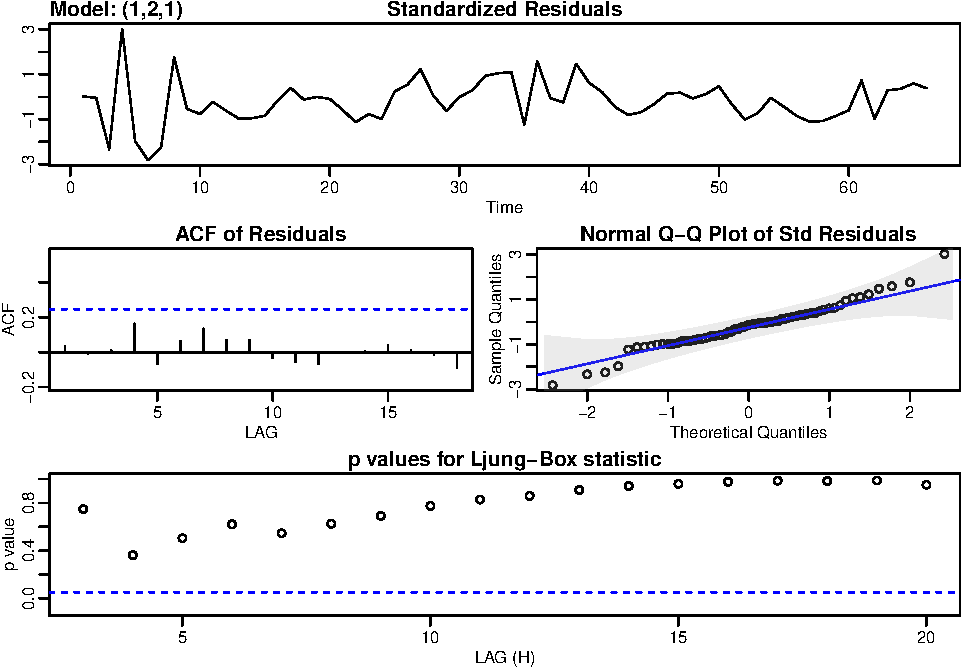
\includegraphics{Q5_files/figure-latex/unnamed-chunk-12-1} \end{center}

\begin{Shaded}
\begin{Highlighting}[]
\NormalTok{seg <-}\StringTok{ }\KeywordTok{c}\NormalTok{(}\KeywordTok{rep}\NormalTok{(}\DecValTok{1}\OperatorTok{:}\DecValTok{5}\NormalTok{, }\DataTypeTok{each=}\DecValTok{11}\NormalTok{), }\KeywordTok{rep}\NormalTok{(}\DecValTok{6}\NormalTok{,}\DecValTok{11}\NormalTok{))}
\KeywordTok{fligner.test}\NormalTok{(model3}\OperatorTok{$}\NormalTok{fit}\OperatorTok{$}\NormalTok{residuals, seg)}
\end{Highlighting}
\end{Shaded}

\begin{verbatim}
## 
##  Fligner-Killeen test of homogeneity of variances
## 
## data:  model3$fit$residuals and seg
## Fligner-Killeen:med chi-squared = 14.177, df = 5, p-value =
## 0.01452
\end{verbatim}

\begin{Shaded}
\begin{Highlighting}[]
\KeywordTok{shapiro.test}\NormalTok{(model3}\OperatorTok{$}\NormalTok{fit}\OperatorTok{$}\NormalTok{residuals)}
\end{Highlighting}
\end{Shaded}

\begin{verbatim}
## 
##  Shapiro-Wilk normality test
## 
## data:  model3$fit$residuals
## W = 0.96917, p-value = 0.09931
\end{verbatim}

\(\;\)

\begin{itemize}
\tightlist
\item
  ARIMA(1, 2, 1)

  \begin{itemize}
  \tightlist
  \item
    Homoscedasticity: the time series of the residuals has no trend and
    the p-value of Fligner's test (0.01452) does not raise much concern.
  \item
    Normality: a few points in the QQplot slightly deviate from the
    straight line resulting in the p-value of Shapiro-Wilk's test
    (0.09931). The normality assumption is valid.
  \item
    White Noise: the p-values of the Ljung-Box statistic are above the
    threshold and there is no concern in the ACF plot. We can safely
    conclude the residuals are realizations of white noise.
  \end{itemize}
\end{itemize}

\newpage

Let's compare the three proposed ARIMA models in terms of their
prediction power using PRESS and MSE.

\begin{Shaded}
\begin{Highlighting}[]
\KeywordTok{par}\NormalTok{(}\DataTypeTok{mfrow=}\KeywordTok{c}\NormalTok{(}\DecValTok{3}\NormalTok{,}\DecValTok{1}\NormalTok{))}
\NormalTok{pred.model1 <-}\StringTok{ }\KeywordTok{sarima.for}\NormalTok{(transformed.covid.training, }\DataTypeTok{n.ahead=}\DecValTok{5}\NormalTok{, }\DataTypeTok{p=}\DecValTok{3}\NormalTok{, }\DataTypeTok{d=}\DecValTok{2}\NormalTok{, }\DataTypeTok{q=}\DecValTok{0}\NormalTok{)}
\NormalTok{pred.model2 <-}\StringTok{ }\KeywordTok{sarima.for}\NormalTok{(transformed.covid.training, }\DataTypeTok{n.ahead=}\DecValTok{5}\NormalTok{, }\DataTypeTok{p=}\DecValTok{0}\NormalTok{, }\DataTypeTok{d=}\DecValTok{2}\NormalTok{, }\DataTypeTok{q=}\DecValTok{1}\NormalTok{)}
\NormalTok{pred.model3 <-}\StringTok{ }\KeywordTok{sarima.for}\NormalTok{(transformed.covid.training, }\DataTypeTok{n.ahead=}\DecValTok{5}\NormalTok{, }\DataTypeTok{p=}\DecValTok{1}\NormalTok{, }\DataTypeTok{d=}\DecValTok{2}\NormalTok{, }\DataTypeTok{q=}\DecValTok{1}\NormalTok{)}
\end{Highlighting}
\end{Shaded}

\begin{Shaded}
\begin{Highlighting}[]
\NormalTok{transformed.covid.test <-}\StringTok{ }\NormalTok{covid.test}\OperatorTok{^}\NormalTok{alpha[}\KeywordTok{which}\NormalTok{(p_values }\OperatorTok{==}\StringTok{ }\KeywordTok{max}\NormalTok{(p_values))]}

\NormalTok{PRESS}\FloatTok{.1}\NormalTok{ <-}\StringTok{ }\KeywordTok{sum}\NormalTok{((pred.model1}\OperatorTok{$}\NormalTok{pred}\OperatorTok{-}\NormalTok{transformed.covid.test)}\OperatorTok{^}\DecValTok{2}\NormalTok{)}
\NormalTok{PRESS}\FloatTok{.2}\NormalTok{ <-}\StringTok{ }\KeywordTok{sum}\NormalTok{((pred.model2}\OperatorTok{$}\NormalTok{pred}\OperatorTok{-}\NormalTok{transformed.covid.test)}\OperatorTok{^}\DecValTok{2}\NormalTok{)}
\NormalTok{PRESS}\FloatTok{.3}\NormalTok{ <-}\StringTok{ }\KeywordTok{sum}\NormalTok{((pred.model3}\OperatorTok{$}\NormalTok{pred}\OperatorTok{-}\NormalTok{transformed.covid.test)}\OperatorTok{^}\DecValTok{2}\NormalTok{)}

\NormalTok{tab =}\StringTok{ }\KeywordTok{rbind}\NormalTok{(}\DecValTok{1}\OperatorTok{:}\DecValTok{3}\NormalTok{, }\KeywordTok{c}\NormalTok{(PRESS}\FloatTok{.1}\NormalTok{, PRESS}\FloatTok{.2}\NormalTok{, PRESS}\FloatTok{.3}\NormalTok{))}
\KeywordTok{row.names}\NormalTok{(tab) =}\StringTok{ }\KeywordTok{c}\NormalTok{(}\StringTok{"ARIMA Model"}\NormalTok{, }\StringTok{"PRESS"}\NormalTok{)}
\KeywordTok{dimnames}\NormalTok{(tab)[[}\DecValTok{2}\NormalTok{]] =}\StringTok{ }\KeywordTok{rep}\NormalTok{(}\StringTok{""}\NormalTok{, }\DecValTok{3}\NormalTok{)}
\NormalTok{tab}
\end{Highlighting}
\end{Shaded}

\begin{verbatim}
##                                        
## ARIMA Model 1.000000 2.000000 3.0000000
## PRESS       6.009946 1.187855 0.1984051
\end{verbatim}

\(\;\)

Based on the PRESS statistic, \textbf{ARIMA(1, 2, 1)} predicts the best.

\(\;\)

\begin{Shaded}
\begin{Highlighting}[]
\NormalTok{MSE}\FloatTok{.1}\NormalTok{ <-}\StringTok{ }\KeywordTok{sum}\NormalTok{((pred.model1}\OperatorTok{$}\NormalTok{pred}\OperatorTok{-}\NormalTok{transformed.covid.test)}\OperatorTok{^}\DecValTok{2}\NormalTok{)}\OperatorTok{/}\DecValTok{3}
\NormalTok{MSE}\FloatTok{.2}\NormalTok{ <-}\StringTok{ }\KeywordTok{sum}\NormalTok{((pred.model1}\OperatorTok{$}\NormalTok{pred}\OperatorTok{-}\NormalTok{transformed.covid.test)}\OperatorTok{^}\DecValTok{2}\NormalTok{)}\OperatorTok{/}\DecValTok{1}
\NormalTok{MSE}\FloatTok{.3}\NormalTok{ <-}\StringTok{ }\KeywordTok{sum}\NormalTok{((pred.model1}\OperatorTok{$}\NormalTok{pred}\OperatorTok{-}\NormalTok{transformed.covid.test)}\OperatorTok{^}\DecValTok{2}\NormalTok{)}\OperatorTok{/}\DecValTok{2}

\NormalTok{tab =}\StringTok{ }\KeywordTok{rbind}\NormalTok{(}\DecValTok{1}\OperatorTok{:}\DecValTok{3}\NormalTok{, }\KeywordTok{c}\NormalTok{(MSE}\FloatTok{.1}\NormalTok{, MSE}\FloatTok{.2}\NormalTok{, MSE}\FloatTok{.3}\NormalTok{))}
\KeywordTok{row.names}\NormalTok{(tab) =}\StringTok{ }\KeywordTok{c}\NormalTok{(}\StringTok{"ARIMA Model"}\NormalTok{, }\StringTok{"MSE"}\NormalTok{)}
\KeywordTok{dimnames}\NormalTok{(tab)[[}\DecValTok{2}\NormalTok{]] =}\StringTok{ }\KeywordTok{rep}\NormalTok{(}\StringTok{""}\NormalTok{, }\DecValTok{3}\NormalTok{)}
\NormalTok{tab}
\end{Highlighting}
\end{Shaded}

\begin{verbatim}
##                                       
## ARIMA Model 1.000000 2.000000 3.000000
## MSE         2.003315 6.009946 3.004973
\end{verbatim}

\(\;\)

Based on the MSE statistic which accounts for the number of parameters,
\textbf{ARIMA(3, 2, 0)} predicts the best.

We choose the superior model to be \textbf{ARIMA(1, 2, 1)} considering
its complexity, PRESS statistic and residuals analysis.

Now, we use the superior model to predict (along with a 95\% prediction
interval) when at least 50\% of the Californians will be fully
vaccinated.

\begin{Shaded}
\begin{Highlighting}[]
\NormalTok{transformed.covid19 <-}\StringTok{ }\NormalTok{covid19}\OperatorTok{^}\NormalTok{alpha[}\KeywordTok{which}\NormalTok{(p_values }\OperatorTok{==}\StringTok{ }\KeywordTok{max}\NormalTok{(p_values))]}

\NormalTok{final.model <-}\StringTok{ }\KeywordTok{sarima.for}\NormalTok{(transformed.covid19, }\DataTypeTok{n.ahead =} \DecValTok{56}\NormalTok{, }\DataTypeTok{p=}\DecValTok{1}\NormalTok{, }\DataTypeTok{d=}\DecValTok{2}\NormalTok{, }\DataTypeTok{q=}\DecValTok{1}\NormalTok{)}
\end{Highlighting}
\end{Shaded}

\begin{Shaded}
\begin{Highlighting}[]
\NormalTok{fit <-}\StringTok{ }\NormalTok{(final.model}\OperatorTok{$}\NormalTok{pred)}\OperatorTok{^}\NormalTok{(}\DecValTok{1}\OperatorTok{/}\FloatTok{0.3}\NormalTok{)}
\NormalTok{lwr <-}\StringTok{ }\NormalTok{(final.model}\OperatorTok{$}\NormalTok{pred}\FloatTok{-1.96}\OperatorTok{*}\NormalTok{final.model}\OperatorTok{$}\NormalTok{se)}\OperatorTok{^}\NormalTok{(}\DecValTok{1}\OperatorTok{/}\FloatTok{0.3}\NormalTok{)}
\NormalTok{upr <-}\StringTok{ }\NormalTok{(final.model}\OperatorTok{$}\NormalTok{pred}\FloatTok{+1.96}\OperatorTok{*}\NormalTok{final.model}\OperatorTok{$}\NormalTok{se)}\OperatorTok{^}\NormalTok{(}\DecValTok{1}\OperatorTok{/}\FloatTok{0.3}\NormalTok{)}

\CommentTok{# data.frame(fit, lwr, upr)}
\end{Highlighting}
\end{Shaded}

\begin{Shaded}
\begin{Highlighting}[]
\KeywordTok{plot}\NormalTok{(covid19,}
     \DataTypeTok{main =} \StringTok{"Fully Vaccinated Californians"}\NormalTok{,}
     \DataTypeTok{xlab =} \StringTok{"Day"}\NormalTok{,}
     \DataTypeTok{ylab =} \StringTok{"Total Vaccinations"}\NormalTok{,}
     \DataTypeTok{xlim =} \KeywordTok{c}\NormalTok{(}\DecValTok{1}\NormalTok{, }\DecValTok{128}\NormalTok{),}
     \DataTypeTok{ylim =} \KeywordTok{c}\NormalTok{(}\DecValTok{0}\NormalTok{, }\DecValTok{25000000}\NormalTok{),}
     \DataTypeTok{type =} \StringTok{"p"}\NormalTok{,}
     \DataTypeTok{pch =} \DecValTok{19}\NormalTok{,}
     \DataTypeTok{col =} \KeywordTok{adjustcolor}\NormalTok{(}\StringTok{"darkgreen"}\NormalTok{, }\FloatTok{0.5}\NormalTok{),}
     \DataTypeTok{xaxt =} \StringTok{"n"}\NormalTok{,}
     \DataTypeTok{yaxt =} \StringTok{"n"}\NormalTok{)}

\KeywordTok{lines}\NormalTok{(}\DataTypeTok{y =}\NormalTok{ fit,}
      \DataTypeTok{x =} \DecValTok{72}\OperatorTok{:}\DecValTok{127}\NormalTok{,}
      \DataTypeTok{type =}\StringTok{"p"}\NormalTok{,}
      \DataTypeTok{pch =} \DecValTok{19}\NormalTok{,}
      \DataTypeTok{col =} \KeywordTok{adjustcolor}\NormalTok{(}\StringTok{"red"}\NormalTok{, }\FloatTok{0.5}\NormalTok{))}

\KeywordTok{lines}\NormalTok{(}\DataTypeTok{y =}\NormalTok{ lwr,}
      \DataTypeTok{x =} \DecValTok{72}\OperatorTok{:}\DecValTok{127}\NormalTok{,}
      \DataTypeTok{type =}\StringTok{"l"}\NormalTok{,}
      \DataTypeTok{pch =} \DecValTok{19}\NormalTok{,}
      \DataTypeTok{col =} \KeywordTok{adjustcolor}\NormalTok{(}\StringTok{"grey"}\NormalTok{, }\FloatTok{0.5}\NormalTok{))}

\KeywordTok{lines}\NormalTok{(}\DataTypeTok{y =}\NormalTok{ upr,}
      \DataTypeTok{x =} \DecValTok{72}\OperatorTok{:}\DecValTok{127}\NormalTok{,}
      \DataTypeTok{type =}\StringTok{"l"}\NormalTok{,}
      \DataTypeTok{pch =} \DecValTok{19}\NormalTok{,}
      \DataTypeTok{col =} \KeywordTok{adjustcolor}\NormalTok{(}\StringTok{"grey"}\NormalTok{, }\FloatTok{0.5}\NormalTok{))}

\KeywordTok{polygon}\NormalTok{(}\KeywordTok{c}\NormalTok{(}\DecValTok{72}\OperatorTok{:}\DecValTok{127}\NormalTok{, }\KeywordTok{rev}\NormalTok{(}\DecValTok{72}\OperatorTok{:}\DecValTok{127}\NormalTok{)), }\KeywordTok{c}\NormalTok{(lwr, }\KeywordTok{rev}\NormalTok{(upr)), }\DataTypeTok{col =} \StringTok{"#69696930"}\NormalTok{, }\DataTypeTok{border =} \OtherTok{NA}\NormalTok{)}
\KeywordTok{abline}\NormalTok{(}\DataTypeTok{h=}\DecValTok{19755000}\NormalTok{, }\DataTypeTok{v=}\DecValTok{127}\NormalTok{, }\DataTypeTok{col=}\StringTok{"blue"}\NormalTok{)}

\KeywordTok{axis}\NormalTok{(}\DataTypeTok{side =} \DecValTok{1}\NormalTok{, }
     \DataTypeTok{at =}\NormalTok{ (}\DecValTok{14}\OperatorTok{*}\DecValTok{0}\OperatorTok{:}\DecValTok{9}\NormalTok{)}\OperatorTok{+}\DecValTok{1}\NormalTok{,}
     \DataTypeTok{cex.axis =} \FloatTok{0.85}\NormalTok{,}
     \DataTypeTok{labels =} \KeywordTok{c}\NormalTok{(}\StringTok{"Jan 12"}\NormalTok{, }\StringTok{"Jan 26"}\NormalTok{, }\StringTok{"Feb 9"}\NormalTok{, }\StringTok{"Feb 23"}\NormalTok{, }\StringTok{"Mar 9"}\NormalTok{, }\StringTok{"Mar 23"}\NormalTok{,}
                \StringTok{"Apr 6"}\NormalTok{, }\StringTok{"Apr 20"}\NormalTok{, }\StringTok{"May 4"}\NormalTok{, }\StringTok{"May 18"}\NormalTok{))}

\KeywordTok{axis}\NormalTok{(}\DataTypeTok{side =} \DecValTok{2}\NormalTok{, }\DataTypeTok{at =}\NormalTok{ (}\DecValTok{5000000}\OperatorTok{*}\DecValTok{0}\OperatorTok{:}\DecValTok{5}\NormalTok{), }\DataTypeTok{labels =} \KeywordTok{c}\NormalTok{(}\StringTok{"0"}\NormalTok{,}\StringTok{""}\NormalTok{,}\StringTok{"10M"}\NormalTok{,}\StringTok{""}\NormalTok{,}\StringTok{"20M"}\NormalTok{, }\StringTok{""}\NormalTok{))}

\KeywordTok{legend}\NormalTok{(}\StringTok{"topleft"}\NormalTok{,}
       \DataTypeTok{lwd =} \DecValTok{2}\NormalTok{,}
       \DataTypeTok{bty =} \StringTok{"n"}\NormalTok{,}
       \DataTypeTok{cex =} \FloatTok{0.8}\NormalTok{,}
       \DataTypeTok{legend =} \KeywordTok{c}\NormalTok{(}\StringTok{"Jan 12 - Mar 23 (Current data)"}\NormalTok{,}
                  \StringTok{"Mar 24 - Mar 18 (Forecast)"}\NormalTok{,}
                  \StringTok{"50% Fully Vaccinated"}\NormalTok{),}
       \DataTypeTok{col =} \KeywordTok{c}\NormalTok{(}\KeywordTok{adjustcolor}\NormalTok{(}\StringTok{"darkgreen"}\NormalTok{, }\FloatTok{0.5}\NormalTok{),}
               \KeywordTok{adjustcolor}\NormalTok{(}\StringTok{"red"}\NormalTok{, }\FloatTok{0.5}\NormalTok{),}
               \KeywordTok{adjustcolor}\NormalTok{(}\StringTok{"blue"}\NormalTok{, }\FloatTok{0.5}\NormalTok{)))}
\end{Highlighting}
\end{Shaded}

\begin{center}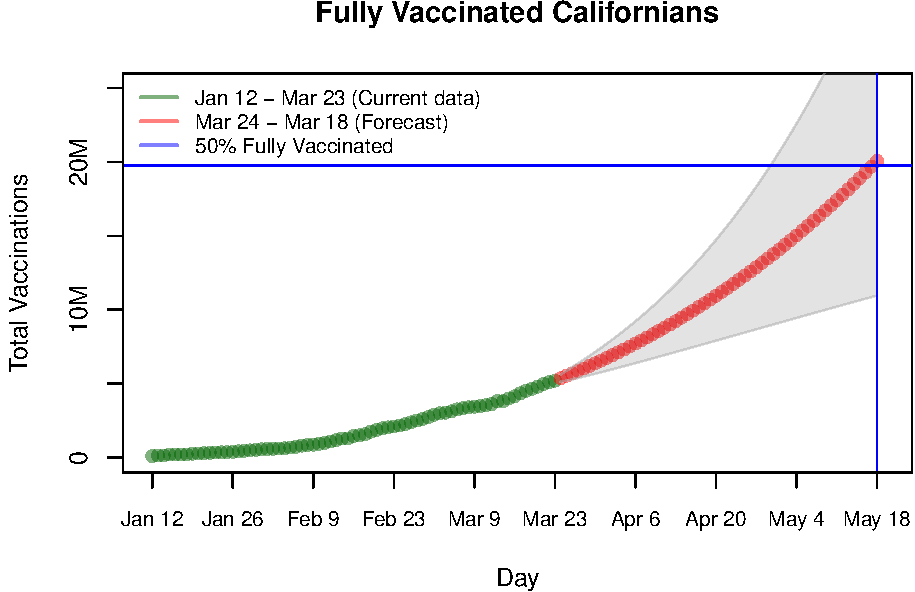
\includegraphics{Q5_files/figure-latex/unnamed-chunk-16-1} \end{center}

According to our model, at least 50\% of Californians
(\textasciitilde{}20M, source: Google) will be fully vaccinated on
\textbf{May 18, 2021}. However, it could be as early as May or as late
as the end of the year (not plotted).

For reference, according to Our World in Data, only 40\% of Californians
(\textasciitilde{}15.5M) have been fully vaccinated as of May 18, 2021.
The most likely reason behind the overestimate is the drop of
Californians that received at least one dose of a vaccine between April
and May (data not included in our dataset). Fewer Californians that
receive at least one dose of a vaccine impact the number of Californians
that become fully vaccinated.


\end{document}
